\documentclass{article}
\usepackage{styles/report}
\usepackage{styles/codespace}

%%%%% Variables %%%%%%
\setprojectname{FitQuest}
\setreportname{Team plan}
\setreportcode{Team-plan-v1.0}
%\setaxilleasrole{fill this in}
%\setbillrole{fill this in}
%\setplatrole{fill this in}
%\sethalvasrole{fill this in}

%\addtolength{\cftsecnumwidth}{52pt}
\renewcommand\thesection{\arabic{section}:}
\renewcommand\thesubsection{\arabic{section}.\alph{subsection}}
\renewcommand\thesubsubsection{\arabic{section}.\alph{subsection}.\roman{subsubsection}}

\reportlayout
\begin{document}
\coverpages


\section{Χρονοπρογραμματισμός}
\vspace{20px}
\subsection{Παραδοχές} 
1.	Για το 1ο παραδοτέο στο Gantt chart αναρτήσαμε τους συντάκτες κάθε τεχνικού κειμένου που συμφωνήθηκαν στην συνάντηση της ομάδας, δεν περιλαμβάνει τα ονόματα των ελεγκτών.
2.	Τα διαγράμματα Gantt και Pert αρχίζουν από τις 20 Μαρτίου που έγινε το πρώτο meeting για την συζήτηση μεθόδου εργασίας.
3.	Κάθε task μελετήθηκε πλήρως ώστε να βρεθεί μια αντιπροσωπευτική εκτίμηση του χρόνου αλλά και τυχόν εξαρτήσεις με άλλα task.
4.	Για λόγους απλότητας και ευελιξίας, κρατήσαμε τις αργίες και τις μέρες Σάββατο Κυριακή μέσα στον χρονοπρογραμματισμό.
\vspace{20px}
\subsection{Διάγραμμα Gantt} 
\begin{center}
    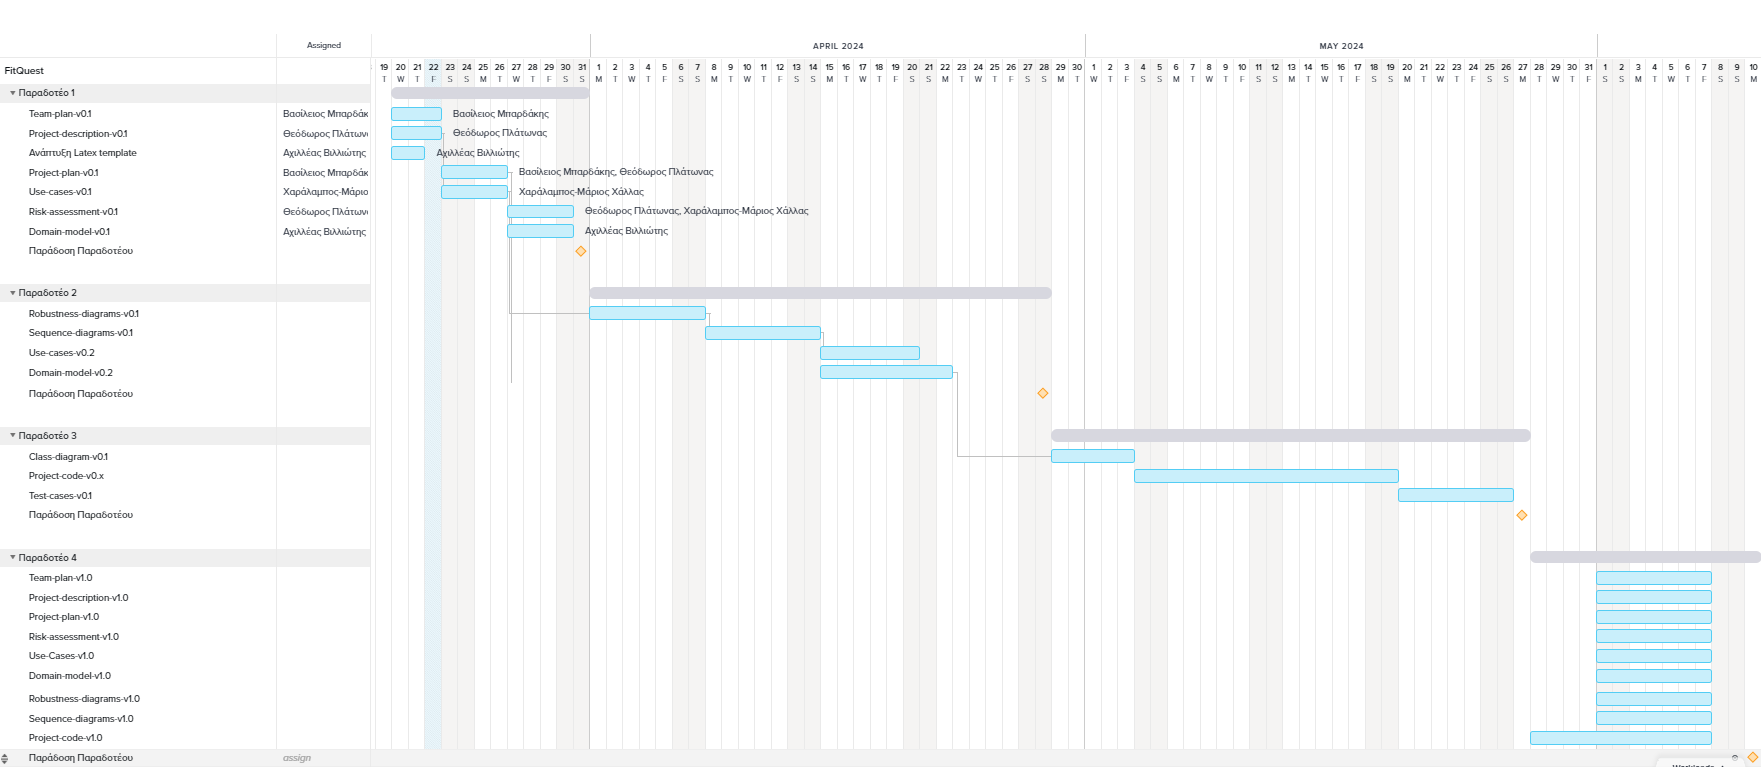
\includegraphics[scale=0.4]{gantteam.png}
\end{center}


\subsection{Διάγραμμα Pert} 

\begin{center}
    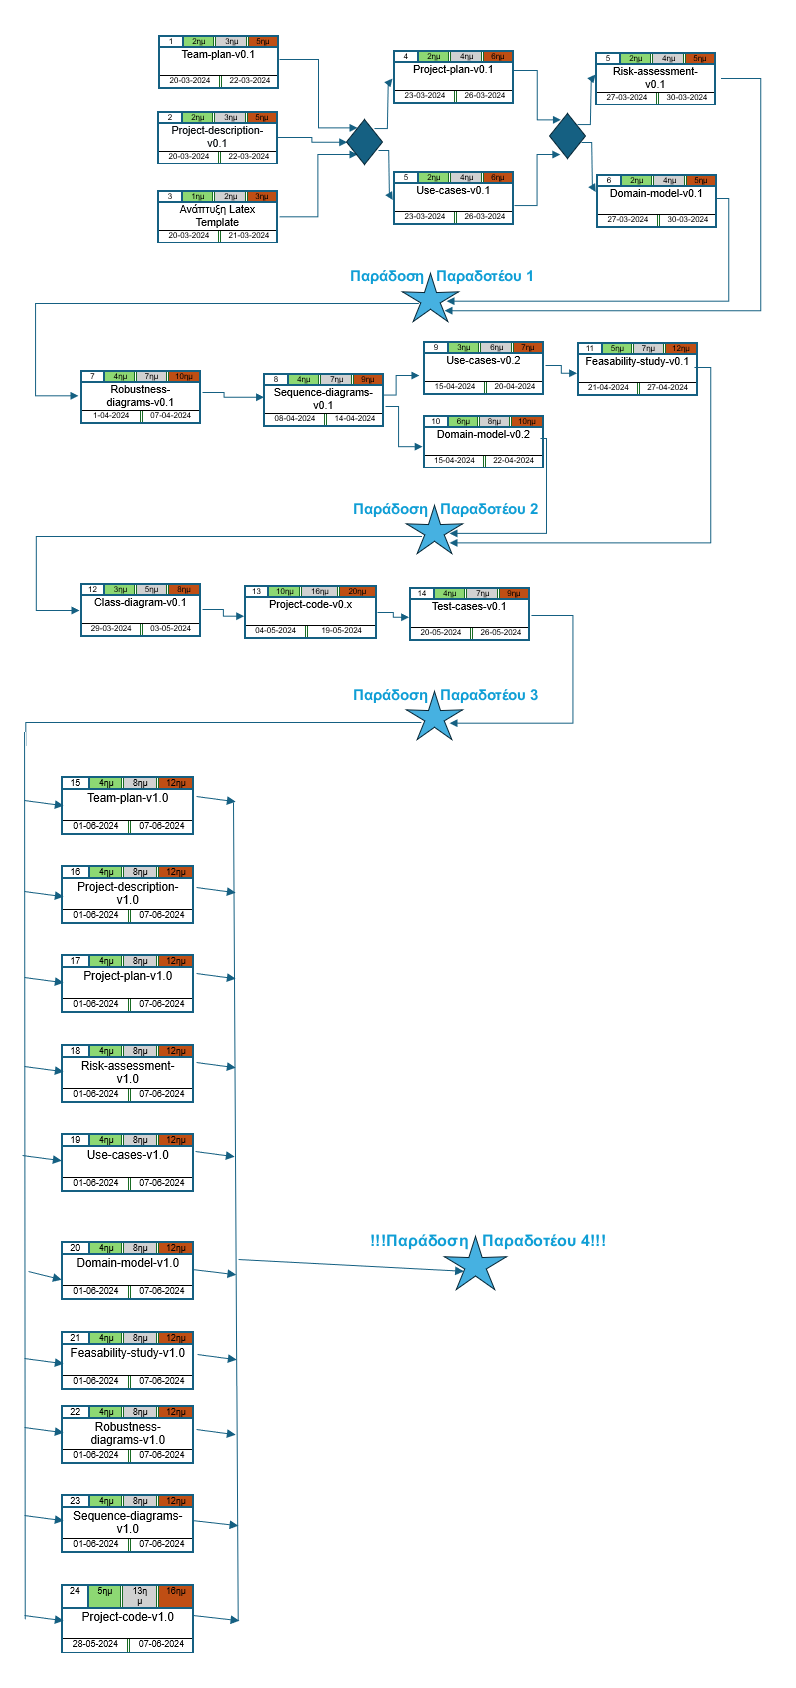
\includegraphics[scale=0.52]{pertteam.png}
\end{center}

\section{Μέθοδος Εργασίας}
Ως ομάδας αποφασίσαμε να εργαστούμε με την μέθοδο Kanban εφόσον είναι εύκολη στην υλοποίηση και διαχείριση για μικρές ομάδες, καθώς και βοηθάει στην ευελιξία που απαιτεί το συγκεκριμένο πρότζεκτ. Αποφασίσαμε ωστόσο να μην έχουμε διακριτούς ρόλους όπως συνηθίζεται με την μέθοδο kanban, και η διαχείριση μέσω των τακτικών meeting. Κάθε τεχνικό κείμενο του παραδοτέου, καθώς και οτιδήποτε άλλο task προκύψει για την υλοποίηση του πρότζεκτ, θα εισάγεται σε μια Kanban κάρτα η οποία θα μπαίνει στον πίνακα της ομάδας. 
Ο πίνακας Kanban της ομάδας στον X άξονα είναι το στάδιο ολοκλήρωσης μιας κάρτας και έχει τα ακόλουθα στάδια: “To Do”, “Working”, “Review” και “Completed”. O άξονας Y είναι η σημαντικότητα μιας κάρτας με τιμές “Υποχρεωτικά”, “Προαιρετικά” και “Extras”, το “Extras” δεν περιέχει τεχνικά κείμενα αλλά διαφορετικά task που χρειάζεται το πρότζεκτ (όπως ανάπτυξη template latex).

\vspace{20px}
\begin{center}
   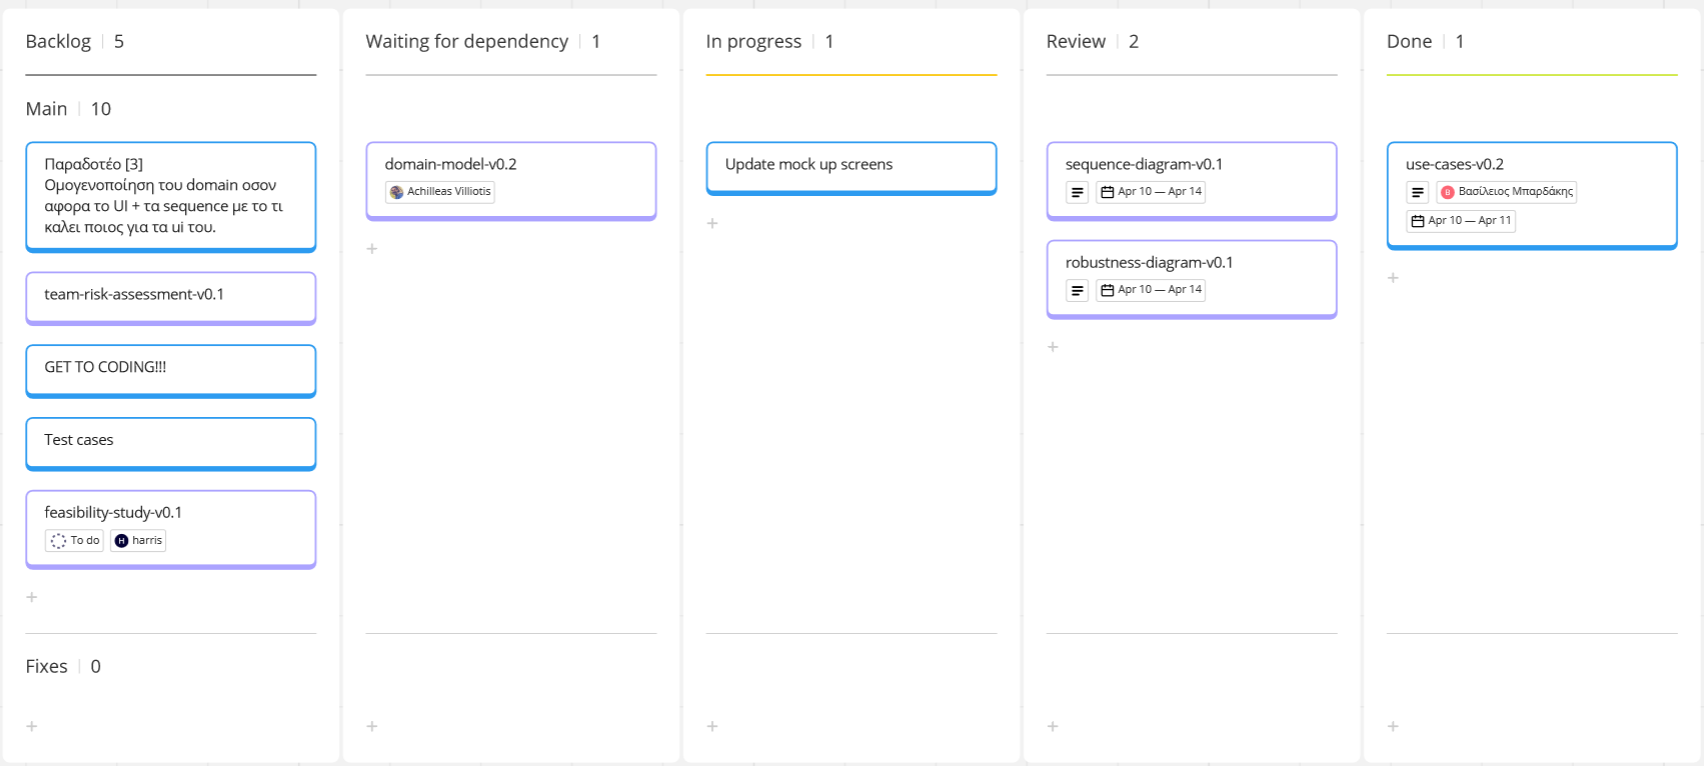
\includegraphics[width=0.9\textwidth]{kanban.png}
\end{center}

\section{Εργαλεία}
Το FitQuest θα αναπτυχθεί σε C\#, σε πρώτη μορφή θα είναι σε desktop έκδοση αλλά επειδή πιθανώς να υπάρξει και mobile έκδοση επιλέξαμε την C\# καθώς και είναι βέλτιστη για cross-platform εφαρμογές. Οι βιβλιοθήκες που θα χρησιμοποιηθούν θα αναφερθούν σε επόμενη έκδοση του τεχνικού κειμένου team-plan.\newline
Διάγραμμα Gant: \href{https://app.teamgantt.com}{app.teamgantt.com}\newline
Διάγραμμα Pert: \href{https://www.microsoft.com/el-gr/microsoft-365/word}{Microsoft Word}\newline
Πίνακας Kanban: \href{www.miro.com}{miro.com}\newline
Διαγράμματα Robustness \& Sequence: \href{https://www.visual-paradigm.com}{visual-paradigm.com}\newline
Προσωρινό royalty free logo: \href{https://www.Vectorstock.com/royalty-free-vector/rpg-creative-icon-from-gaming-icons-collection-vector-45969591}{vectorstock.com}
\textbf{



\end{document}
